我们提出的PointNet网络结构(\ref{sec:pointnet_arch}节)的灵感主要来源于\ref{sec:point_set_property}节所述的$\mathbb{R}^n$内点集的属性。 % We first describe the three properties in Sec~\ref{sec:point_set_property}; accordingly, we discuss our architecture designs in Sec~\ref{sec:pointnet_arch}, where we also summarize our whole network for classification and segmentation tasks. Furthermore, Sec~\ref{sec:theory} provides some theoretical analysis on how and why our network works well on point sets, though the architecture is not complicated.

\subsection{$\mathbb{R}^n$内点集的属性}
\label{sec:point_set_property}
网络的输入是来自欧几里得空间的点的子集,主要有一下三种主要的性质:

% \begin{itemize}
\bitem
\item 无序性。
不同于图片的像素或者立方体的体素,点云是一些无特定顺序的点的集合。换句话说,一个要处理$N$个3D点集的网络需要对按序输入的点集的$N!$种排序保持不变。 
\item 点之间有相互作用。这些点来自具有距离度量的空间。这意味着这些点不是孤立的,而且相邻的点形成一个具有意义的子集。因此,模型需要能够从邻近点中捕获局部结构,以及局部结构之间的组合相互作用。 
\item 转换的不变性。
作为一个几何体,已习得的点集表示需要对一些变换保持不变。例如,对一些点一起做旋转和平移变换既不会改变全局的点云类别、也不会改变点的分割。
\eitem
% \end{itemize}

% The above three properties of our input lead to the three key ideas of our network design, which are discussed respectively in the following section.


\subsection{PointNet的结构}
\label{sec:pointnet_arch}

我们的完整网络架构图如图\ref{fig:pointnet_arch}所示,其中用于分类的网络和用于分割的网络占据了网络结构中的很大一部分。请阅读图\ref{fig:pointnet_arch}的题注以了解流程。

我们的网络有三个关键模块:用作对称函数、聚类所有点的信息的最大池化层;一个局部和全局信息结合的结构;和两个对齐了输入点和点的特征的联合对齐网络。

我们将在以下的单独段落中讨论这些设计选择背后的原因。%, after a brief overview of the network.

% \paragraph{Overview} In basic PointNet: Given a point cloud input, for example, $n$ points of $(x,y,z)$ coordinates, the network firstly applies a function (multi-layer perceptron network) on each point independently. Function outputs across points are then aggregated with a max pooling layer. The aggregated vector is a global feature for the point cloud.
% 
% For classification task, the global feature is further passed through a few fully connected layers (with ReLU) to predict class scores for the entire point cloud.
% 
% For segmentation, we need to combine both local and global context for point class prediction. To this end, the global feature is appended to each point's local feature vector to provide a global context for individual point. We then apply a multi-layer perceptron net on the concatenated feature of each point to predict its class scores.
% 
% Additional input and feature space alignment network can be inserted, as shown in Fig~\ref{fig:pointnet_arch}. The alignment network is a regressor to transformation matrix and resembles the basic classification net in architecture.
% 

\paragraph{用于处理无序输入的对称函数}
为了使模型对输入排序不变,存在三种策略:1)将输入排列为规范顺序;2)将输入看作训练RNN的序列,但通过各种排列增加了训练数据;3)用一个简单的对称函数来聚类每个点的信息。这里,对称函数将$n$个向量作为输入,然后输出一个不受输入顺序变化影响的新向量。例如,$+$和$*$操作符是对称二元函数。 

尽管排序听起来像是一个简单的解决方法,但实际上谈及到一般意义上的点的扰动时,在高维空间中并不存在稳定的排序。这可以很容易地通过矛盾来显示。如果这样一种排序策略存在,那么它定义了高维空间和一维实线之间的双向映射。不难看出,谈及点扰动时要求排序的稳定等同在维度降低时保持映射在空间上的接近度,一般情况下这项任务是无法实现的。因此,排序并不能完全解决排序问题,而且因为排序问题的存在,网络很难学习到从输入到输出的一致映射。如实验(图\ref{fig:order_invariant})中所示,我们发现直接在排序点集上应用多层感知机的性能不好,尽管略优于直接处理无序输入。

使用RNN的方法是将点集作为顺序信号,并希望用随机排序的序列训练RNN,这样RNN将会变得和输入顺序无关。然而,在``OrderMatters''~\cite{vinyals2015order}中,作者已经证明顺序确实很重要而且无法完全被忽略。尽管RNN对于较短(几十个)的序列的输入排序已经具有相对良好的鲁棒性,但是很难扩展到像点集这样有成千上万的输入元素上。根据实验,我们也证明了基于RNN的模型在性能上不如我们所提出来的方法(图\ref{fig:order_invariant})。

我们的想法是通过对集合中转换元素应用对称函数来近似在点集上定义的一般函数:
\begin{align}
    f(\{x_1, \dots, x_n\})\approx g(h(x_1), \dots, h(x_n)),
    \label{eq:approx}
\end{align}
其中 $f:2^{\mathbb{R}^N} \rightarrow \mathbb{R}$, $h: \mathbb{R}^N\rightarrow \mathbb{R}^K$ 和 $g:\underbrace{\mathbb{R}^K\times \dots \times \mathbb{R}^K}_n \rightarrow \mathbb{R}$ 是对称函数。

根据实验,我们的基础模块十分简单:我们通过多层感知机来近似$h$,并通过单个变量函数和最大池化函数的组合来近似$g$。通过实验发现这样的模块结构表现的很好。通过$h$的集合,我们可以学到一些$f$来捕获点集的不同属性。 % This idea shares similar flavor with [cite leo's paper: probablistic shape fingerprint], where they define random functions on the input data and train a model based on the outputs of those optimization functions.  %Signature points are supposed to result in more extreme values for those random functions, thus the latter model can use weights to select them to make prediciton decisions for specific tasks. 
% In our architecture, instead of using random functions, we let the network itself learn a set of optimal functions to select signature points. 

尽管我们的关键模块看起来很简单,但它也具有很精彩的地方(参见\ref{sec:visualizing_pointnet}节),在一些不同的应用中能够表现出很强的性能(参见\ref{sec:application}节)。由于我们模块的简单性,我们也提供了\ref{sec:theory}节中的理论分析。


\paragraph{局部和全局信息聚类}
上一节的输出组成了一个向量$[f_1, \dots, f_K]$,这是输入集的全局标签。我们可以在形同全局特征上很容易训练SVM或多层感知机分类器以进行分类。然而,点的分割需要结合局部信息和全局信息。我们能够通过简单而高效的方式来实现这一目标。 % Even for global point classification, it could be beneficial to exploit more local geometries.

我们的解决方法可以在图\ref{fig:pointnet_arch}(\textit{Segmentation Network})中看到。在计算完全局点云特征向量后,我们将全局特征和每一个点的特征连接起来反馈给每一个点特征。然后我们基于组合的点特征提取新的每个点的特征,这样每个点特征都考虑了局部和全局信息。 % This structure can be repeated multiple times.

通过这样的修改,我们的网络能够预测依赖于局部几何和全局语义的每个点数量。例如我们可以准确地预测出每个点的法线(图中的补充),验证网络能够汇总来自该点的局部领域的信息。在实验环节中,我们也表明我们的模型可以在形状部分分割和场景分割方面实现最先进的性能。
    
\paragraph{联合对齐网络}
如果点云在经历了某些几何变换(比如刚性变换),那么点云的语义标签必须是不变的。因此我们希望已习得的点集表示不受这些变换影响。

一个自然的解决方法是在特征提取前将所有的输入集对齐到规范空间。Jaderberg等人~\cite{jaderberg2015spatial}介绍了一种通过采样和插值来对齐二维图像的空间变换的方法,通过在GPU上特别定制的层来实现。

与~\cite{jaderberg2015spatial}相比,我们的点云输入形式使我们能够以更简单的方式来实现这一目标。我们不需要发明任何新的层,也不需要像图像任务那样引入任何别名。我们通过一个小型网络(图~\ref{fig:pointnet_arch}中的T-net)预测仿射变换矩阵,并直接将该变换作用于输入点的坐标。这一小型网络本身类似于大型网络,由独立的点特征提取、最大池化和全连接层组成。更多关于T-net的细节将在附录中介绍。

这个想法可以进一步扩展到特征空间的对齐。我们可以在点的特征上插入另一个对齐网络,并预测特征变换矩阵以对齐来自不同输入点云的特征。然而,特征空间中的变换矩阵比空间变换矩阵的维度高很多,这极大地增加了优化的难度。因此,我们在softmax的训练损失中增加了一个正则化项。我们约束特征变换矩阵接近于正交矩阵:
\begin{equation}
    L_{reg} = \|I - AA^T\|_F^2,
\end{equation}
其中$A$是小型网络预测得到的特征对齐矩阵。正如我们所期待的,一个正交变换将不会损失任何输入的信息。我们发现通过增加正则化项,优化变得更加稳定,而且我们的模型实现了更好的性能。


\subsection{理论分析}
\label{sec:theory}
 
% \todo{
%   goal: show that this network is theoretically robust to perturbation and corruption (additional points and incompleteness) of input data.
%   \begin{itemize}
%     \item analyze the max pooling layer: it selects a finite set of key points. the cardinality of the key point set is constrained by the dimension of max pooling. 
%     \item add some understanding of the symmetry function, if we can
%   \end{itemize}
% }

\paragraph{通用近似性} 

我们首先展示我们的神经网络具备通用近似到连续的集合函数上的能力。由于集函数的连续性,直观上我们认为,一个输入点集上的微小扰动不应当引起函数值的剧烈变化,例如其分类任务或分割任务的表现分数。

%We first show the universal approximation ability of our neural network to continuous set functions. By the continuity of set functions, intuitively, a small perturbation to the input point set should not greatly change the function values, such as classification or segmentation scores.

形式化地, 令 $\mathcal{X}=\{S: S\subseteq [0,1]^m \text{ and } |S|=n\}$,   $f:\mathcal{X}\rightarrow \mathbb{R}$ 在 $\mathcal{X}$ 上关于赫斯多夫距离 $d_H(\cdot, \cdot)$ (即: $\forall \epsilon > 0, \exists \delta >0$, for any $S, S'\in\mathcal{X}$, if $d_H(S, S') < \delta$, 则有 $|f(S)-f(S')|< \epsilon$)的连续的集函数。 我们的理论认为在池化层给定足够多的神经元, $f$ 能被无限近似,即, 在 \eqref{eq:approx} 中的 $K$ 
已经足够大。

% Formally, let $\mathcal{X}=\{S: S\subseteq [0,1]^m \text{ and } |S|=n\}$,   $f:\mathcal{X}\rightarrow \mathbb{R}$ is a continuous set function on $\mathcal{X}$ w.r.t to Hausdorff distance $d_H(\cdot, \cdot)$, i.e., $\forall \epsilon > 0, \exists \delta >0$, for any $S, S'\in\mathcal{X}$, if $d_H(S, S') < \delta$, then $|f(S)-f(S')|< \epsilon$. Our theorem says that $f$ can be arbitrarily approximated by our network given enough neurons at the max pooling layer, i.e., $K$ in \eqref{eq:approx} is sufficiently large. 

\begin{theorem}

令 $f:\mathcal{X}\rightarrow \mathbb{R}$ 是一个关于赫斯多夫距离 $d_H(\cdot, \cdot)$ 的集函数。$\forall \epsilon > 0$, $\exists$ 一个连续函数 $h$ 和一个对称函数 $g(x_1, \dots, x_n)=\gamma \circ \mbox{MAX}$, 使得任意 $S\in\mathcal{X}$,

% Suppose $f:\mathcal{X}\rightarrow \mathbb{R}$ is a continuous set function w.r.t Hausdorff distance $d_H(\cdot, \cdot)$. $\forall \epsilon > 0$, $\exists$ a continuous function $h$ and a symmetric function $g(x_1, \dots, x_n)=\gamma \circ \mbox{MAX}$, such that for any $S\in\mathcal{X}$,


\begin{align*}
	\left|f(S) - \gamma\left(\underset{x_i\in S}{\mbox{MAX}}\left\{h(x_i)\right\}\right)\right| < \epsilon
\end{align*}

其中 $x_1, \ldots, x_n$ 是一系列在 $S$ 中任意顺序排列的元素,$\gamma$ 是一个连续函数, 且 $\mbox{MAX}$ 是一个取 $n$ 个向量最为输入,然后返回一个元素层面上的最大值的最大化向量运算符。

\end{theorem}

该定理的理论证明参见本文的附加材料。其主要思想是,在最差情况下,通过将空间划分成等体积的体素,网络的学习结果是到将点云转换为体积表示。而在实际情况下,网络会学习一个聪明得多的策略来探测空间,正如我们将在点函数的可视化中呈现的那样。

% The proof to this theorem can be found in our supplementary material. The key idea is that in the worst case the network can learn to convert a point cloud into a volumetric representation, by partitioning the space into equal-sized voxels. In practice, however, the network learns a much smarter strategy to probe the space, as we shall see in point function visualizations.

\begin{figure}[t!]
    \centering
    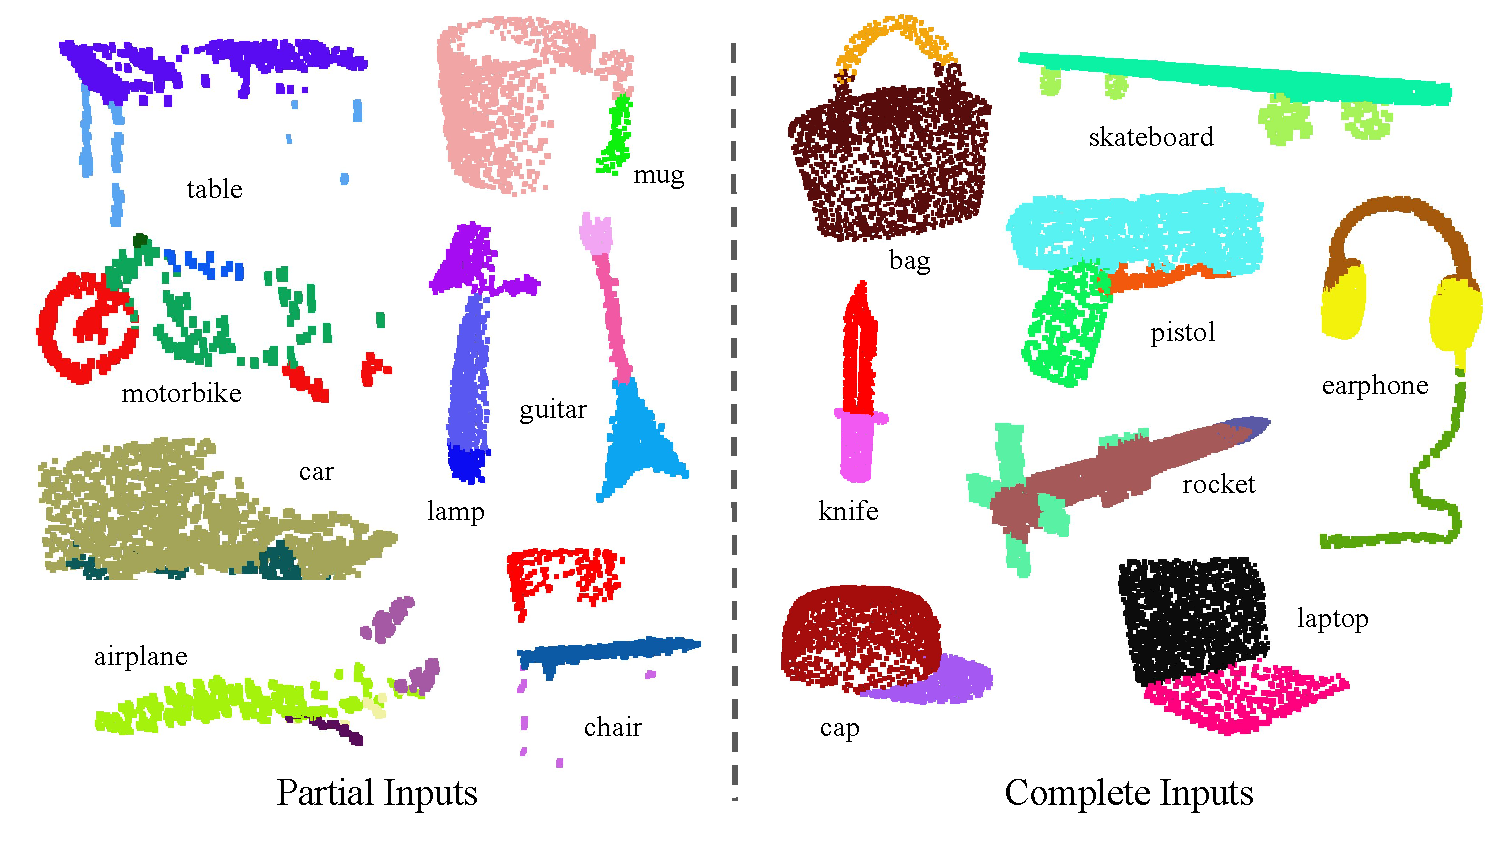
\includegraphics[width=0.8\linewidth]{fig/segres.pdf}
    \caption{
        \textbf{零件分割的量化结果} 我们可视化了横跨 16 个分类的 CAD 零件的分割结构。我们分别展示了部分模拟的 Kinect 扫描结果(左)和完全的 ShapeNet CAD 模型的结果(右)。
  %  \textbf{Qualitative results for part segmentation.} We visualize the CAD part segmentation results across all 16 object categories. We show both results for partial simulated Kinect scans (left block) and complete ShapeNet CAD models (right block).
    }
    \label{fig:qualitative_part_segmentation}
\end{figure}

\paragraph{瓶颈维度与稳定性} 从理论上和实践上,我们发现我们网络的表达性收到池化层维度的强烈影响。即,\eqref{eq:approx} 中的 $K$。在此我们提供了一个分析,同时也揭示了与我们模型的稳定性相关的一些属性。  

% \paragraph{Bottlenet dimension and stability} Theoretically and experimentally we find that the expressiveness of our network is strongly affected by the dimension of the max pooling layer, i.e., $K$ in \eqref{eq:approx}. Here we provide an analysis, which also reveals properties related to the stability of our model. 

我们定义 $\myvec u=\underset{x_i\in S}{\mbox{MAX}}\{h(x_i)\}$ 为网络 $f$ 的子网络。其中 $f$ 将分布在  $[0,1]^m$ 中的点集映射到了 $K$ 维空间的向量。接下来的理论分析指出,输入中的微小扰动或额外的噪音点不会严重影响我们网络的输出结果。

%We define $\myvec u=\underset{x_i\in S}{\mbox{MAX}}\{h(x_i)\}$ to be the sub-network of $f$ which maps a point set in $[0,1]^m$ to a $K$-dimensional vector. The following theorem tells us that small corruptions or extra noise points in the input set are not likely to change the output of our network:

\begin{theorem}

令 $\myvec u:\mathcal{X}\rightarrow \mathbb{R}^K$ 使得 $\myvec u=\underset{x_i\in S}{\mbox{MAX}}\{h(x_i)\}$ 且 $f=\gamma \circ \myvec u$. 则, 

% Suppose $\myvec u:\mathcal{X}\rightarrow \mathbb{R}^K$ such that $\myvec u=\underset{x_i\in S}{\mbox{MAX}}\{h(x_i)\}$ and $f=\gamma \circ \myvec u$. Then, 

\begin{enumerate}[label=(\alph*)]   

    \item $\forall S, \exists~\mathcal{C}_S, \mathcal{N}_S\subseteq \mathcal{X}$,  $f(T)=f(S)$ if  $\mathcal{C}_S\subseteq T\subseteq \mathcal{N}_S$;
    %\item Define the equivalence relation $\sim$ as $S\sim S'$ if $\myvec u(S)=\myvec u(S')$, then $\mathcal{C}_S=\underset{S'\sim S}{\cap} S'$ and $\mathcal{N}_S=\underset{S'\sim S}{\cup} S'$.
    % \item Let $S\sim S'$ if $\myvec u(S)=\myvec u(S')$. $\mathcal{C}_S=\underset{S'\sim S}{\cap} S'$, $\mathcal{N}_S=\underset{S'\sim S}{\cup} S'$.
    \item $|\mathcal{C}_S| \le K$
\end{enumerate}
\label{thm:thm2}
%     \begin{itemize}            
%     \item Critical points.
%     \\$\mathbb{C}=\{x_i: \myvec u_j(S)=h_j(x_i) \mbox{ for some } 1\le j\le K\}\cap S$
%     \item Free-space points.
%     \\$\mathbb{F}=\{x_i: \myvec u_j(S)<h_j(x_i) \mbox{ for some } 1\le j\le K\}\cap S$
%     \item Non-critical points. 
%     \\$\mathbb{N}=\{x_i: \myvec u_j(S)>h_j(x_i) \mbox{ for some } 1\le j\le K\}\cap S$
% For any $S'$ such that  $\mathbb{C} \subseteq S' \subseteq \mathbb{C}\cup\mathbb{N}$, $\myvec u(S')\equiv \myvec u(S)$; for any $S'$ such that $S'\cap \mathbb{F}\neq \emptyset$, $\myvec u(S')\neq \myvec u(S)$.
%\end{itemize}
\end{theorem}

关于上述定理,我们进一步阐释其推论。(a) 说明 $f(S)$ 在针对输入干扰时保持不变,只要  $\mathcal{C}_S$ 中的点被保留。同时也不会受到在 $\mathcal{N}_S$ 以内的额外噪声点的影响。(b) 说明 $\mathcal{C}_S$ 只包含一些有限数量的点,取决于 \eqref{eq:approx} 中的 $K$。换句话说,$f(S)$ 事实上是完全由一个元素数量小于或等于 $K$ 的有限子集 $\mathcal{C}_S\subseteq S$决定的。因此,我们将 $\mathcal{C}_S$ 称为 $S$ 的 \emph{关键点集},将 $K$ 成为 $f$ 的 \emph{瓶颈维度}。

% We explain the implications of the theorem. (a) says that $f(S)$ is unchanged up to the input corruption if all points in $\mathcal{C}_S$ are preserved; it is also unchanged with extra noise points up to $\mathcal{N}_S$. (b) says that $\mathcal{C}_S$ only contains a bounded number of points, determined by $K$ in \eqref{eq:approx}. In other words, $f(S)$ is in fact totally determined by a finite subset $\mathcal{C}_S\subseteq S$ of less or equal to $K$ elements. We therefore call $\mathcal{C}_S$ the \emph{critical point set} of $S$ and $K$ the \emph{bottleneck dimension} of $f$. 

结合 $h$ 的连续性,我们的模型关于点的扰动、缺失或额外的噪声点的健壮性得以解释。其健壮性的提升类似于机器学习模型中的稀疏原则。\textbf{直观上看,我们的模型能够通过一个稀疏的关键点来概括出形状。}在实验部分,我们可以看到从一个物体骨架的关键点。

% Combined with the continuity of $h$, this explains the robustness of our model w.r.t point perturbation, corruption and extra noise points. The robustness is gained in analogy to the sparsity principle in machine learning models. {\bf  Intuitively, our network learns to summarize a shape by a sparse set of key points.} In experiment section we see that the key points form the skeleton of an object.




\begin{comment}
\subsection{The properties of point sets in $\R^n$}
\todo{
  our input is a subset of points from a Euclidean space. It has three main properties:
  \begin{itemize}
    \item as a set, points in it has no order; 
    \item the points are from a metric space. therefore, local structures from near points have to be characterized;
    \item as a geometric object, the learned representation of the point set should be invariant to certain transformations.
  \end{itemize}
  the above three properties of our input leads to the three key ideas of our network design. we explain one by one.
}
\subsection{Unordered point set as input}
\todo{
  \begin{itemize}
    \item three strategies exist: 1) sorting input into a canonical order; 2)  use RNN but train order-invariantly; 3) use a symmetric function to aggregate the information from each point. 
    \item theoretically and empirically argue that the first two choices are not good. 
    \item our idea is to approximate a general function defined on a point set by applying a symmetric function on transformed elements in the set: $$f(\{x_1, \dots, x_n\})\approx g(h(x_1), \dots, h(x_n)),$$ where $f:2^{\R^N} \rightarrow \R$, $h: \R^N\rightarrow \R$ and $g:\R\times \dots \times \R\rightarrow \R$ is a symmetric function.
    \item we think this is provable for some good $f$.
    \item empirically, we approximate $h$ by a multi-layer perceptron network and $g$ by a composition of a single variable function and a max pooling function. this is found to work well by experiments.
    \item we can learn a number of $f$'s to capture different properties of the set.
  \end{itemize}
}

\subsection{Local and global information aggregation}
\todo{
  \begin{itemize}
    \item the output from the above section forms a vector $[f_1, \dots, f_M]$, which is a global signature of the input set.
    \item however, for tasks such as segmentation, we also need combine local information and global information. 
    \item xxx
  \end{itemize}
}

\subsection{Input and feature space alignment}
\todo{
  \begin{itemize}
    \item as we explained earlier, the learned representation of the point set should be invariant to certain transformations.
    \item we propose to apply an input dependent transformation for each instance to align all input set to a canonical space
    \item the input of our data are very friendly to geometric transformations, such as affine. we can therefore predict the transformation matrix by a neural network, named Joint Alignment Network.
    \item this idea can be extended to the alignment of feature space, as well
  \end{itemize} 
}

\subsection{PointNet architecture}
\todo{
  \begin{itemize}
    \item we implement the above ideas into a network for point set learning, named PointNet
    \item show the network for classification and explain 
    \item show the network for segmentation and explain
  \end{itemize}
}

\subsection{Theoretical Analysis}
\todo{
  goal: show that this network is theoretically robust to perturbation and corruption (additional points and incompleteness) of input data.
  \begin{itemize}
    \item analyze the max pooling layer: it selects a finite set of key points. the cardinality of the key point set is constrained by the dimension of max pooling. 
    \item add some understanding of the symmetry function, if we can
  \end{itemize}
}



\end{comment}